\documentclass[10pt,a4paper]{article}
\usepackage[utf8]{inputenc}
\usepackage[top=1.25in, bottom=1.25in, left=.75in, right=.75in]{geometry}
\usepackage{amsmath}
\usepackage{algorithmicx}
\usepackage{algpseudocode}
\usepackage{algorithm2e}
\usepackage{amsfonts}
\usepackage{mathtools}
\usepackage{amssymb}
\usepackage{xcolor}
\usepackage{natbib}
\usepackage{bibentry}
\usepackage{float}
\usepackage{fancyhdr}
\usepackage{dsfont}
\usepackage{graphicx,caption}
\renewcommand{\familydefault}{\sfdefault}
\pagestyle{fancy}
\lhead{Exercise sheet \#4}
\rhead{Johannes Ender, MNr.: 01629746}
%\nobibliography*
\DeclareMathOperator*{\argmax}{arg\,max}
\author{Johannes Ender}
\begin{document}
\section{Functional Approximation}
\subsection*{46. Autonomous Orchard}
\begin{align*}
\vec{w} = \begin{pmatrix} w_1 \\ w_2 \\ w_3\end{pmatrix}, \vec{S}=\begin{pmatrix} A \\ B \\ C\end{pmatrix},\\ \hat{v}(\vec{w}, \vec{S}) = w_1 \cdot A + w_2 \cdot B + w_3 \cdot C,\\ \nabla \hat{v}(\vec{w}, \vec{S}) = \begin{pmatrix} A \\ B \\ C\end{pmatrix} \\ \\
\text{$1^{st}$ step:}\\
w_1 &= w_0 + \alpha [G - \hat{v}(\vec{w_0}, \vec{S_0})]\nabla \hat{v}(\vec{w_0}, \vec{S_0}) \\
&= \begin{pmatrix} 0 \\ 0 \\ 0\end{pmatrix} + 0.01 [3 - (0\cdot 4 + 0 \cdot 7 + 0 \cdot 1)]\begin{pmatrix} 4 \\ 7 \\ 1\end{pmatrix} \\
&= \begin{pmatrix} 0.12 \\ 0.21 \\ 0.03\end{pmatrix} \\ \\
\text{$2^{nd}$ step:}\\
w_2 &= w_1 + \alpha [G - \hat{v}(\vec{w_1}, \vec{S_1})]\nabla \hat{v}(\vec{w_1}, \vec{S_1}) \\
&= \begin{pmatrix} 0.12 \\ 0.21 \\ 0.03\end{pmatrix} + 0.01 [-15 - (0.12\cdot 10 + 0.21 \cdot 6 + 0.03 \cdot 0)]\begin{pmatrix} 10 \\ 6 \\ 0\end{pmatrix} \\
&= \begin{pmatrix} -1.626 \\ -0.838 \\ 0.03\end{pmatrix} \\ \\
\text{$3^{rd}$ step:}\\
w_3 &= w_2 + \alpha [G - \hat{v}(\vec{w_2}, \vec{S_2})]\nabla \hat{v}(\vec{w_2}, \vec{S_2}) \\
&= \begin{pmatrix} -1.626 \\ -0.838 \\ 0.03\end{pmatrix} + 0.01 [5 - -(1.626\cdot 20 + (-0.838) \cdot 1 + 0.03 \cdot 15)]\begin{pmatrix} 10 \\ 6 \\ 0\end{pmatrix} \\
&= \begin{pmatrix} 5.956 \\ -0.459 \\ 5.716\end{pmatrix} \\ \\
\text{$4^{th}$ step:}\\
w_4 &= w_3 + \alpha [G - \hat{v}(\vec{w_3}, \vec{S_3})]\nabla \hat{v}(\vec{w_3}, \vec{S_3}) \\
&= \begin{pmatrix} 5.956 \\ -0.459 \\ 5.716\end{pmatrix} + 0.01 [21 - (5.956\cdot 4 + (-0.459) \cdot 19 + 5.716 \cdot 3)]\begin{pmatrix} 4 \\ 19 \\ 3\end{pmatrix} \\
&= \begin{pmatrix} 5.505 \\ -2.6 \\ 5.38\end{pmatrix}
\end{align*}
Additional to the calculations by hand, they were implemented as the Python script \texttt{autonomous\_orchard.py} to cross-check the results.

\newpage
\subsection*{47. Exercise 9.1 Show that tabular methods such as presented in Part I of this book are a special case of linear function approximation. What would the feature vectors be?}

\subsection*{48. Exercise 10.4 Give pseudocode for a differential version of semi-gradient Q-learning.}
\RestyleAlgo{boxruled}
\begin{algorithm}[ht]
\textbf{Initialize:}
$\vec{w}, \vec{R}, S$\\
	\For{ each step}
	{
		choose $A$ as a function of $\hat{q}(S, \cdot , \vec{w})$ (e.g. $\epsilon$ -greedy)\\
		take action $A$ and observe $R, S'$ \\
		$\delta \leftarrow R-\overline{R} + max_a \hat{q}(S', a, \vec{w}) - \hat{q}(S, A, \vec{w})$\\
		$\vec{R} \leftarrow \vec{R} + \beta \delta$\\
		$\vec{w} \leftarrow \vec{w} + \alpha \delta \nabla q(S, A, \vec{w})$\\
		$S \leftarrow S'$
	}	
 \caption{Differential semi-gradient Q-learning}
\end{algorithm}

\subsection*{49. Exercise 11.1 Convert the equation of n-step off-policy TD (7.9) to semi-gradient form. Give accompanying definitions of the return for both the episodic and continuing cases.}
Using the definitions:
\begin{align*}
G_{t:t+n} \doteq R_{t+1} + \gamma R_{t+2} + \cdots + \gamma^{n-1}R_{t+n} + \gamma^n \hat{v} (S_{t+n}, w_{t+n-1})\end{align*}
for the episodic case and
\begin{align*}
G_{t:t+n} \doteq R_{t+1} - {R}_t + R_{t+2} - \overline{R}_{t+1} + \cdots + R_{t+n} - \overline{R}_{t+n-1} + \hat{v}(S_{t+1}, w_{t+n-1})
\end{align*}
for the continuous case, one can write the n-step off-policy TD in semi-gradient form as
\begin{align*}
w_{t+n} = w_{t+n-1} + \alpha \rho_{t:t+n-1}[G_{t:t+n} - \hat{v}(S_t, w_{t+n-1})]\nabla \hat{v}(S_t, w_{t+n-1})
\end{align*}


\subsection*{50. Exercise 12.1 Just as the return can be written recursively in terms of the first reward and itself one-step later (3.9), so can the $\lambda$-return. Derive the analogous recursive relationship from (12.2) and (12.1).}
\newpage
\subsection*{51. Implementation Task: Reinforce}
See Exercise 52 for result figurej and file \texttt{reinforce.py} for the implementation.
\subsection*{52. Implementation Task: Reinforce with Baseline}
As environment to run the implemented REINFORCE algorithm against, the CartPole-v0 environment of the OpenAI gym framework was chosen.\\
Strangely, the variant with baseline performs worse than the variant without baseline. The used approximation for the value-function was a simple pre-calculated array containing the the discounted values of the states at certain time steps. This could be done, as per default, the maximum number of time steps of this environment is 200.
\begin{figure}[H]
\centering
\captionsetup{width=.5\linewidth}
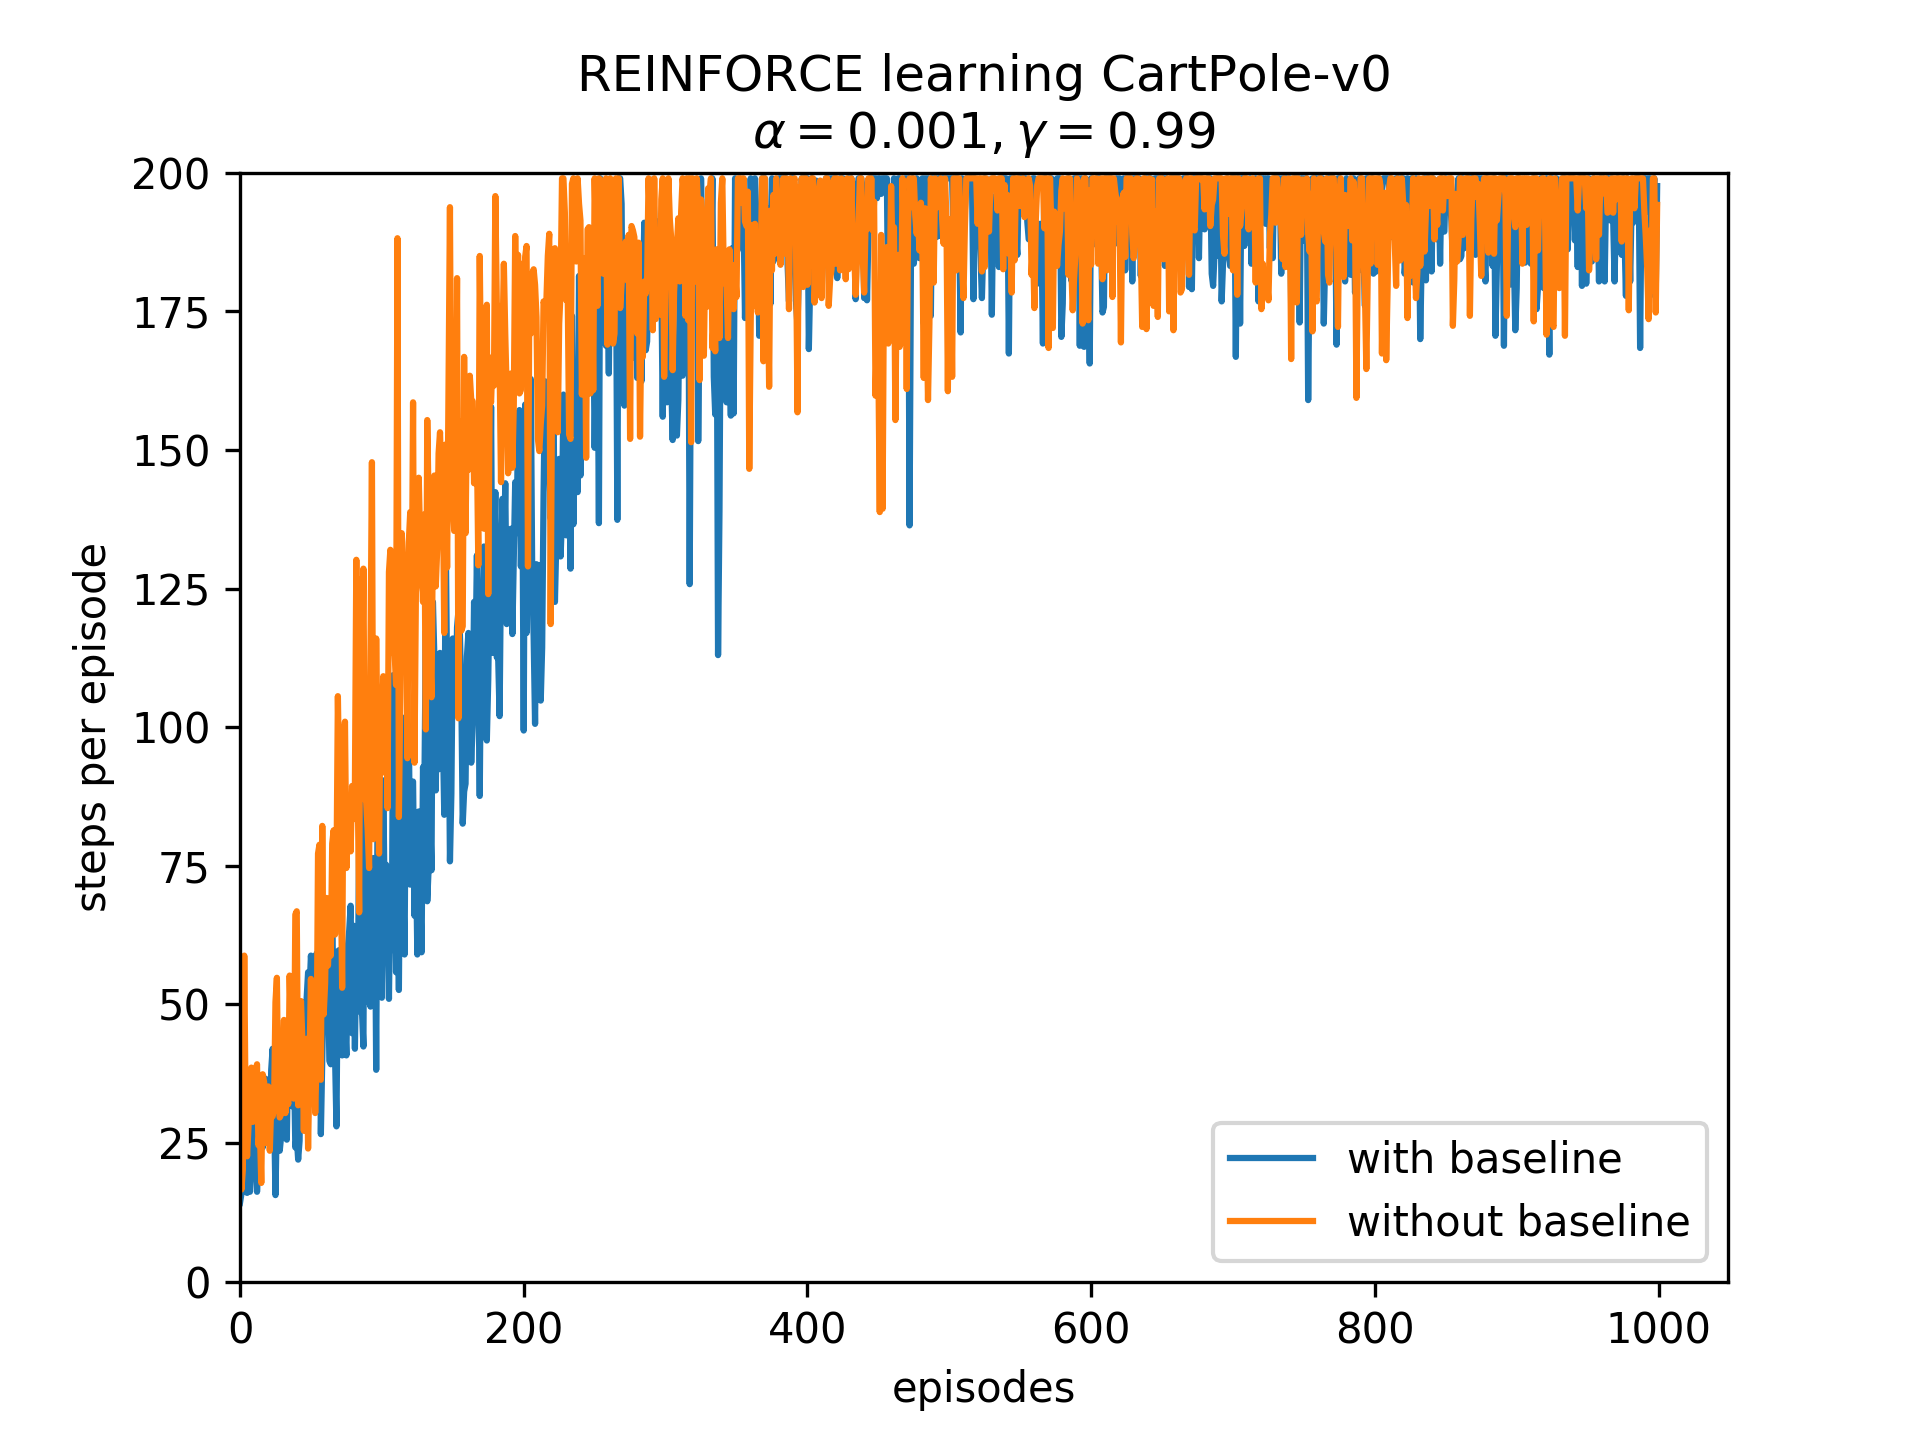
\includegraphics[width=.5\linewidth]{./REINFORCE_cartpole.png}
\caption{Comparison of steps taken per episode for learning the cartpole-v0 problem from the OpenAI gym environment using the REINFORCE algorithm once with baseline and without baseline.The shown results are averaged over 5 runs.}
\end{figure}


Results were generated using the file \texttt{reinforce.py}.
\subsection*{53. Implementation Task: Actor-Critic}
Not implemented.
\subsection*{54. Implementation Task: Step-Size Parameter}
To check what happens, when the condition $\sum_{n=1}^\infty = \alpha_n^2 < \infty$, the SARSA algorithm and the WindyGridWorld environment implemented in the previous exercise set were used. The program was run once with the step size $\alpha$ set to 0.5 and once to 1.5. On can see in Figure 2, that if $\alpha=0.5$, the algorithm rather quickly converges, but if the step size is increased to 1.5, it never converges. The shown figure only goes up to 1000 episodes, but simulations were run longer and no change to the behavior was observed.
\begin{figure}[H]
\centering
\captionsetup{width=.5\linewidth}
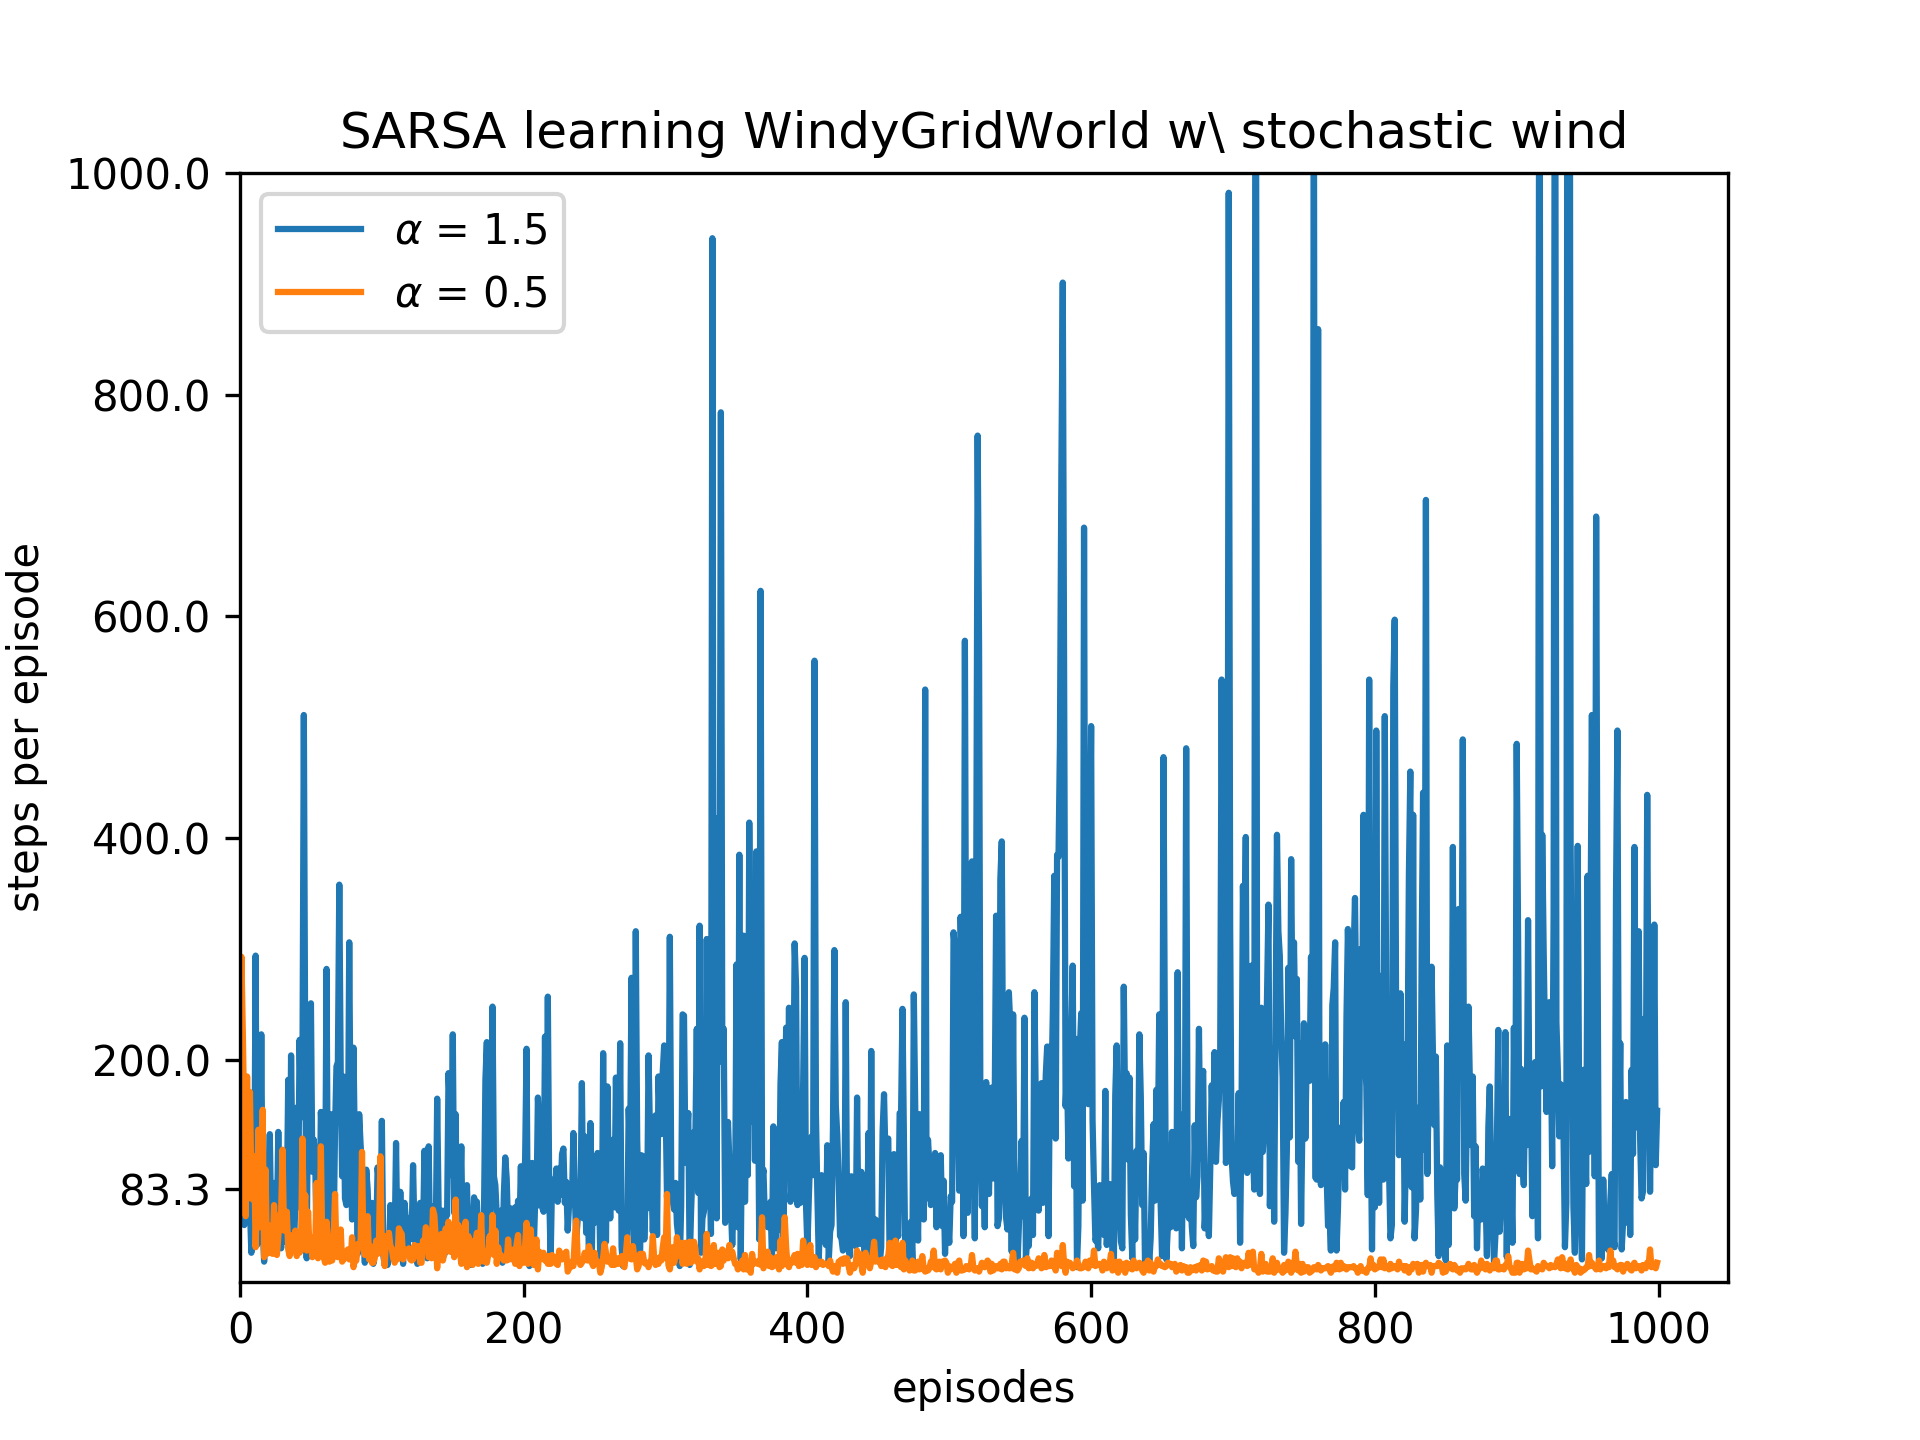
\includegraphics[width=.5\linewidth]{./WindyGridWorld_stochastic_wind.png}
\caption{Comparison of steps taken per episode for learning the cartpole-v0 problem from the OpenAI gym environment using the REINFORCE algorithm once with baseline and without baseline.}
\end{figure}
\end{document}